\documentclass[tikz,border=10pt]{standalone}
\begin{document}
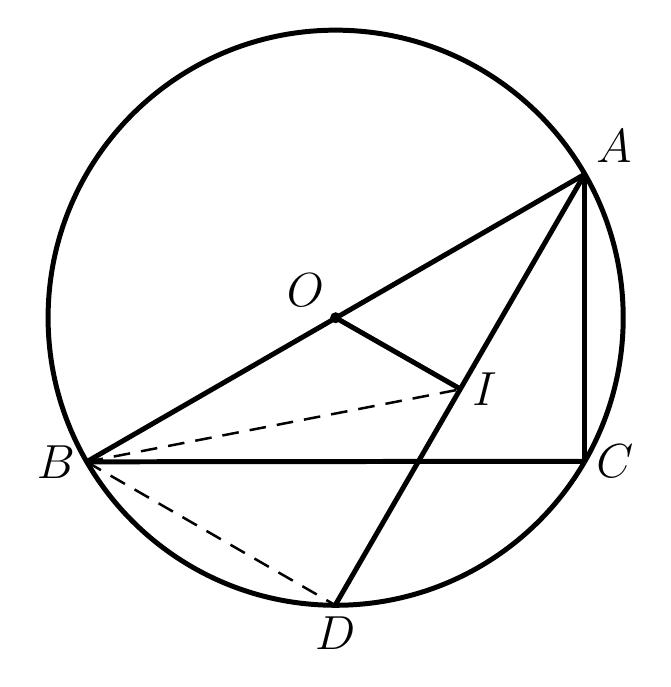
\begin{tikzpicture}[line join=round, line width=1.8pt]
\coordinate (A) at (3.160,2.259);
\coordinate (B) at (-3.164,-1.392);
\coordinate (C) at (3.160,-1.385);
\coordinate (D) at (-0.006,-3.212);
\coordinate (O) at (-0.001,0.438);









\coordinate (I) at (1.588,-0.470);


\draw (O) circle[radius=3.652];


\draw (A) -- (B);
\draw (B) -- (C);
\draw (A) -- (D);
\draw (A) -- (C);
\draw (O) -- (I);


\draw[dash pattern=on 6pt off 4pt, line width=0.9pt] (B) -- (D);
\draw[dash pattern=on 6pt off 4pt, line width=0.9pt] (B) -- (I);


\fill (O) circle[radius=2.000pt];


\node[above right, font=\fontsize{18}{21.6}\selectfont] at (A) {$A$};
\node[left,        font=\fontsize{18}{21.6}\selectfont] at (B) {$B$};
\node[right,       font=\fontsize{18}{21.6}\selectfont] at (C) {$C$};
\node[below,       font=\fontsize{18}{21.6}\selectfont] at (D) {$D$};
\node[above left,  font=\fontsize{18}{21.6}\selectfont] at (O) {$O$};
\node[right,       font=\fontsize{18}{21.6}\selectfont] at (I) {$I$};
\end{tikzpicture}
\end{document}